\subsection{Constant}
\label{subsec:pd:constant}


% ----------------------- paths to graphics ------------------------

\graphicspath{{5_automatic_learning/pattern_detection/images/}}

% ----------------------- contents from here ------------------------
% 

The \nameref{subsec:pd:constant} pattern detector identifies columns that have (mostly) a single value. We refer to these columns as being constant. An additional parameter is provided in the initialization: \(constant\_ratio_{min}\) which indicates the minimum ratio of the constant value, based on which a column is considered constant or not. This pattern detector works on all data types, therefore the \textit{select\_column} method always returns \textit{True}. This is a single-column pattern detector and columns are evaluated independently. The next paragraphs describe the pattern detection process for a single column.

The \textit{scanning} phase is responsible for building the histogram of values on the column. The \textit{evaluation} phase selects the most common value \(C\) as the constant candidate---the value with the highest number of occurrences. The \(constant\_ratio\) of the column represents the evaluation metric and is computed as follows:
\begin{equation}
\label{eq:pd:constant:constantratio}
    constant\_ratio = \frac{count_{C}}{count_{notnull}}
\end{equation}
where:
\begin{itemize}
    \item[] \(count_{C}\) = number of occurrences of the constant candidate \(C\)
    \item[] \(count_{notnull}\) = number of non-null values in the column
\end{itemize}

The column is considered to fit the \nameref{subsec:pd:constant} pattern if the \(constant\_ratio\) is greater or equal to \(constant\_ratio_{min}\). All values that are not equal to \(C\) are considered exceptions. The \textit{evaluation result} is composed of the \textit{coverage} and \textit{row\_mask}---as defined in \ref{subsec:genericpd}~\nameref{subsec:genericpd}---and the \(constant\_ratio\) as an additional pattern-specific result. The metadata needed for compression and decompression is the constant \(C\).

The \textit{expression nodes} for the \nameref{subsec:pd:constant} pattern are illustrated in Figure~\ref{fig:pd:constant:exprnode}.

\begin{figure}[h]
  \centering
  \begin{subfigure}[t]{0.4\linewidth}
    \centering
    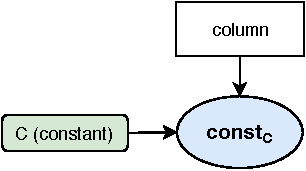
\includegraphics[width=0.8\linewidth]{expression_node-constant-compression_2.pdf}
    \caption[b]{compression}
    \label{fig:pd:constant:exprnode:compression}
  \end{subfigure}
  \hspace{1em}
  \begin{subfigure}[t]{0.4\linewidth}
    \centering
    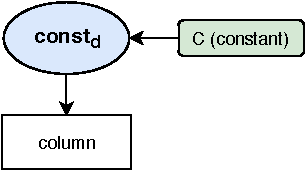
\includegraphics[width=0.8\linewidth]{expression_node-constant-decompression_2.pdf}
    \caption[b]{decompression}
    \label{fig:pd:constant:exprnode:decompression}
  \end{subfigure}
  \caption{Constant expression nodes}
  \label{fig:pd:constant:exprnode}
\end{figure}

The \textit{compression node} takes as input the constant column and does not generate any output column. Similarly, the \textit{decompression node} does not require any column to produce the constant column.

The compression and decompression operators are \(const_{c}\) and \(const_{d}\). The metadata they require is the constant \(C\). \(const_{c}\) takes as input a value \(v\) and checks whether it is equal to \(C\). If \textit{True}, then it returns nothing. Else, it raises an \textit{OperatorException} indicating that \(v\) is an exception and should be added to the exception column. \(const_{d}\) does not take any input value and returns the constant \(C\).

The benefit of the \nameref{subsec:pd:constant} representation scheme is clear: we avoid storing a column on disk. Dictionary encoding could also be used to compress constant columns, however it still stores a column with dictionary ids as opposed to no column at all. A more generic alternative representation for constant columns would be a \textit{whitebox} version of RLE that supports any data types.

% ---------------------------------------------------------------------------
% ----------------------- end of thesis sub-document ------------------------
% ---------------------------------------------------------------------------
